\chapter{Estimating Range}
As the name Frequency Modulated Continuous Wave (FMCW) implies, a FMCW radar is
a continuous time system which transmits and receives a periodic signal whose 
frequency has been modulated. As a periodic signal, the transmitted signal has
the complex form (with unit-normalized amplitude)
\begin{equation}
	\label{eq:complex-sinusoid}
	p(t) = e^{j2\pi f(t)t}.
\end{equation}
The typical frequency modulation used in FMCW radar systems is the sawtooth
modulation, given by
\cite{iovescufundamentals, wang2008digital}
\begin{equation}
	\label{eq:sawtooth}
	f(t) = f_c + \alpha (t - kT_c), \quad\text{for } kT_c \leq t < (k+1)T_c, \quad
	k \in \mathbb{Z}
\end{equation}
where $\alpha > 0$ is the chirp-rate  $\frac{df}{dt}$, $f_c$ is the base
carrier frequency (e.g. 77 GHz), and $T_c$ is the period of the chirp. To
simplify the calculations, we will deal with a single chirp until for range
calculations, thus the frequency for a single chirp is 
\begin{equation}
	f(t) = f_c + \alpha t \quad\text{for } 0\leq t < T_c.
\end{equation}

The maximum frequency of each chirp is 
\begin{equation}
	f_{max} \triangleq f_c + \alpha T_c,
\end{equation}
and the bandwidth $B$ of the signal is
\begin{equation}
	B = f_{max} - f_c = \alpha T_c.
\end{equation}

Combining the sawtooth frequency modulation (\ref{eq:sawtooth}) with the complex
sinusoid (\ref{eq:complex-sinusoid}), we get
the transmitted (TX) signal as
\begin{equation}
	p(t) = e^{j(2\pi f_c t+ \pi \alpha t^2)}.
\end{equation}

\begin{figure}[h]
	\centering
	\begin{subfigure}[b]{0.8\textwidth}
		\begin{tikzpicture}
			\begin{axis}[
			axis x line = bottom,
			axis y line = left,
			xlabel = $t$,
			ylabel=$f(t)$,
			xmin=0, xmax=8,
			ymin=0, ymax=3.2,
			xtick=\empty,
			ytick=\empty,
			xlabel near ticks,
			ylabel near ticks,
			extra x ticks={4,8},
			extra x tick labels={$T_c$, $2T_c$},
			extra y ticks={0, 1, 3},
			extra y tick labels={$0$, $f_c$, $f_{max}$},
			]
			\draw 
				(axis cs:1.5, 1.75)
				-| (axis cs:2, 2)
				node [near end, right]
				{$\alpha$};
			\addplot [
			domain=0:8,
			samples=100,
			color=black,
			]
			{(1 + 0.5*x)*(x<4)+(1+0.5*(x-4))*(x>4)};
			\end{axis}
		\end{tikzpicture}
		\label{fig:sawtooth}
		\caption{Example of sawtooth frequency modulation}
	\end{subfigure}
	\begin{subfigure}[b]{0.8\textwidth}
		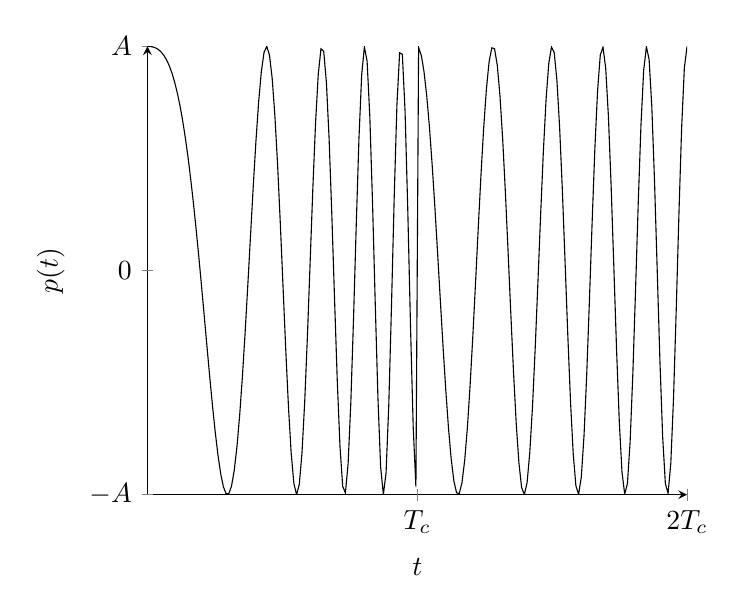
\begin{tikzpicture}
			\begin{axis}[
			axis x line = bottom,
			axis y line = left,
			xlabel = $t$,
			ylabel=$p(t)$,
			xmin=0, xmax=8,
			ymin=-1, ymax=1,
			xtick=\empty,
			ytick=\empty,
			xlabel near ticks,
			ylabel near ticks,
			extra x ticks={4,8},
			extra x tick labels={$T_c$, $2T_c$},
			extra y ticks={-1, 0, 1},
			extra y tick labels={$-A$, $0$, $A$},
			]
			\addplot [
			domain=0:8,
			samples=200,
			color=black,
			]
			{cos(deg(2*pi*((0.125 + 0.25*x)*(x<4)+(0.25+0.125*(x-4))*(x>4))*x)};
			\end{axis}
		\end{tikzpicture}
		\label{fig:pulse}
		\caption{Example of TX signal $p(t)$}
	\end{subfigure}
\end{figure}

Consider a target at a distance $d$ from the radar, such that the transmitted
(RX) signal reflects off the target and returns to the radar. This received signal
will be a time delayed version of the TX signal, where the time delay $\tau$ is
given by
\begin{equation}
	\tau = \frac{2d}{c}
\end{equation}
where $c$ is the speed of light. The RX signal thus has the form
\begin{equation}
	p(t-\tau)=e^{j(2\pi f_c (t-\tau) + \pi\alpha (t-\tau)^2)}.
\end{equation}

\begin{figure}[h]
	\centering
	\begin{tikzpicture}
		\begin{axis}[
		axis x line = bottom,
		axis y line = left,
		xlabel = $t$,
		ylabel=$f(t)$,
		xmin=0, xmax=8,
		ymin=0, ymax=3.2,
		xtick=\empty,
		ytick=\empty,
		xlabel near ticks,
		ylabel near ticks,
		extra x ticks={1,4,8},
		extra x tick labels={$\tau$,$T_c$, $2T_c$},
		extra y ticks={0, 1, 1.5, 3},
		extra y tick labels={$0$, $f_c$, $f_b$, $f_{max}$},
		]
		\draw[dashed] (axis cs:0, 1.5) -| (axis cs:1, 0);
			
		\addplot [
		domain=0:8,
		samples=100,
		color=black,
		]
		{(1 + 0.5*x)*(x<4)+(1+0.5*(x-4))*(x>4)};
		\addplot [
		domain=0:8,
		samples=100,
		color=red,
		]
		{(x<1)*1 + (1+0.5*(x-1))*(x>1)*(x<5) + (1+0.5*(x-5))*(x>5)};
		\end{axis}
	\end{tikzpicture}
	\label{fig:received}
	\caption{Frequency of RX signal (delayed by time $\tau$)}
\end{figure}

To recover $\tau$, and subsequently $d$, we define a new dechirped signal $r(t)$
as the product of the transmitted signal with the complex conjugate of the
received signal
\begin{align}
	r(t) &\triangleq p(t)p^*(t-\tau) \\
	&= e^{j(2\pi f_c t + \pi \alpha t^2)}e^{-j[2\pi f_c (t-\tau) + \pi\alpha (t-\tau)^2 ]} \\
	&= e^{j(2\pi f_c \tau - \pi \alpha \tau^2)}e^{j2\pi\alpha\tau t}.\label{eq:range}
\end{align}
Note, the first exponential in (\ref{eq:range}) only depends on $\tau$, so it is
a constant phase term. However, the second term varies according to a constant
frequency (named the beat frequency) $f_b$
\begin{equation}
	f_b \triangleq \alpha \tau.
\end{equation}
Recovering $f_b$ allows us to recover the distance $d$ as
\begin{equation}
	\label{eq:distance}
	d = \frac{c f_b}{2\alpha}
\end{equation}
The maximum beat frequency occurs when $\tau = T_c$, as any $\tau \in (T_c, 2T_c]$ will
appear as $\tau^*$
\begin{equation}
	\tau^* = \tau - T_c, \quad \tau \in (T_c, 2T_c]
\end{equation}
and thus the recovered distance $d^*$ will be less than the true range the
target is from the radar. From this, we can get our maximum recoverable distance
for a given chirp period
\begin{equation}
	d_{max} = \frac{c T_c}{2}.
\end{equation}
To recover the beat frequency $f_b$ from the dechirped signal, $r(t)$, we can
simply use the Fourier Transform to get
\begin{align}
	R_r(f) &= \int_{-\infty}^{\infty} r(t) e^{-j2 \pi ft} dt \label{eq:range-ft}\\
	&= \int_{-\infty}^{\infty} e^{j(2\pi f_c \tau - \pi \alpha \tau^2)}e^{j2\pi\alpha\tau t} e^{-j2\pi ft}dt\\
	&= e^{j(2\pi f_c \tau - \pi \alpha
	\tau^2)}\int_{-\infty}^{\infty}e^{-j2\pi(f - \alpha\tau ) t} dt\\
	&= e^{j(2\pi f_c \tau - \pi \alpha \tau^2)}\delta (f - \alpha \tau),
\end{align}
where $\delta(f)$ is the Dirac Delta function.

Now consider the case of multiple ($N$) objects at different distances $d_i$ from the radar.
\begin{equation}
	d_i \not = d_j \quad \text{for } i \not = j, \quad i,j \in [1, N]
\end{equation}
Each of these objects will reflect the transmitted chirp with a unique delay
$\tau_i$, and therefore will have a unique beat frequency corresponding to these
delays. Using the continuous time Fourier Transform, we can always resolve the
unique beat frequencies corresponding to the time delays. 

\begin{figure}[h]
	\centering
	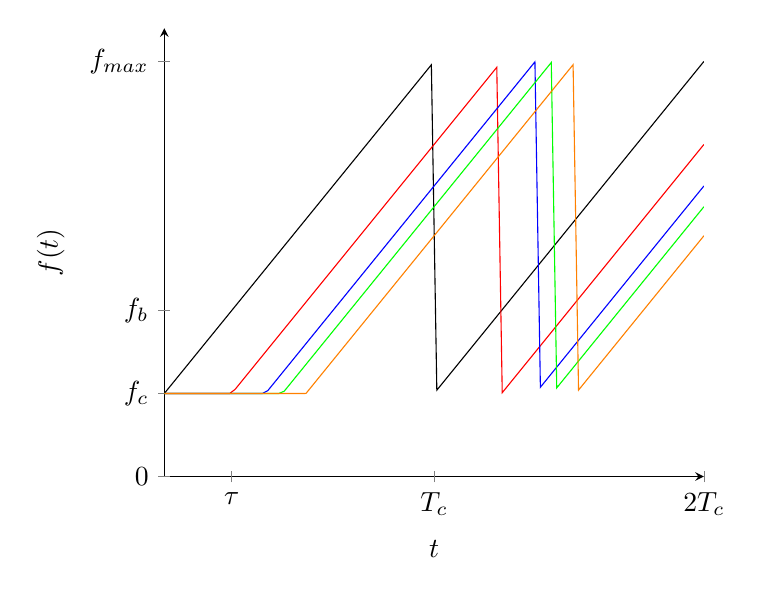
\begin{tikzpicture}
		\begin{axis}[
		axis x line = bottom,
		axis y line = left,
		xlabel = $t$,
		ylabel=$f(t)$,
		xmin=0, xmax=8,
		ymin=0.5, ymax=3.2,
		xtick=\empty,
		ytick=\empty,
		xlabel near ticks,
		ylabel near ticks,
		extra x ticks={1,4,8},
		extra x tick labels={$\tau$,$T_c$, $2T_c$},
		extra y ticks={0.5, 1, 1.5, 3},
		extra y tick labels={$0$, $f_c$, $f_b$, $f_{max}$},
		]
		\addplot [
		domain=0:8,
		samples=100,
		color=black,
		]
		{(1 + 0.5*x)*(x<4)+(1+0.5*(x-4))*(x>4)};
		\addplot [
		domain=0:8,
		samples=100,
		color=red,
		]
		{(x<1)*1 + (1+0.5*(x-1))*(x>1)*(x<5) + (1+0.5*(x-5))*(x>5)};
		\addplot [
		domain=0:8,
		samples=100,
		color=blue,
		]
		{(x<1.5)*1 + (1+0.5*(x-1.5))*(x>1.5)*(x<5.5) +
			(1+0.5*(x-5.5))*(x>5.5)};
		\addplot [
		domain=0:8,
		samples=100,
		color=green,
		]
		{(x<1.75)*1 + (1+0.5*(x-1.75))*(x>1.75)*(x<5.75) +
			(1+0.5*(x-5.75))*(x>5.75)};
		\addplot [
		domain=0:8,
		samples=100,
		color=orange,
		]
		{(x<2.1)*1 + (1+0.5*(x-2.1))*(x>2.1)*(x<6.1) +
			(1+0.5*(x-6.1))*(x>6.1)};
		\end{axis}
	\end{tikzpicture}
	\label{fig:received}
	\caption{Frequencies of reflected signals from multiple objects}
\end{figure}

However, in practice we must sample the received signal $r(t)$ with an
Analog-to-Digital converter (ADC), with sampling frequency $f_s = 1/T_s$. To retrieve
the beat frequencies, we take the $M$-point Discrete Fourier Transform (DFT) of
$r(t)$ for each chirp period
\begin{align}
	R_r[f] &= \sum_{m=0}^{M-1} r[mT_s] e^{-j\frac{2\pi}{M}fm} \label{eq:range-fft}\\
	&= \sum_{m=0}^{M-1} e^{j(2\pi f_c\tau -
	\pi\alpha\tau^2)}e^{j2\pi\alpha\tau mT_s} e^{-j\frac{2\pi}{M}fm}.
\end{align}
From this, we can see $R_r[f]$ has a peak when $f=MT_s\alpha\tau$, and since
$M$, $T_s$, and $\alpha$ are configured parameters, we can recover $\tau$ and
subsequently the distance $d$.
This processing can be done efficiently on hardware with the Fast Fourier Transform (FFT),
so this step is often called the Range-FFT. 

Since we are using the DFT, we can only resolve frequency components
separated by $1/T_c$, as $T_c$ is the observation window,
\begin{equation}
	\Delta f > \frac{1}{T_c}.	
\end{equation}
From (\ref{eq:distance}), we get the range-cell resolution
\begin{align}
	\Delta d &= \frac{c\Delta f}{2\alpha}\\
	\implies \Delta d &> \frac{c}{2\alpha T_c} = \frac{2}{2B}. \label{eq:range-res}
\end{align}

